\section{Ancillary Measurements}

We discuss in this section a number of ancillary measurements that are not central to the primary goal of measuring the photo-detector positions but are a valuable by-product of the x-ray position measurement technique. 

\subsection { X-ray interaction rate -- 2017 vs 2018}  
The efficacy of spacer materials between MPPC, PCB strip and CFRP
plate is tested by examining the X-ray event rate as a function of
MPPC position. The rate is inversely proportional to the length of LXe
traversed by the X-ray before interaction.  It provides crucial
information about the state of spacer materials responsible for
preventing LXe leak between inner cryostat wall and the photosensitive
surface, which directly impacts photo detection and reconstruction
efficiencies, and energy response.  A constant rate of triggered
events is expected from all scanned MPPCs with some variation
attributed to electronic readouts that are nominally configured in an
identical way.  The event rates show a $\phi$ dependent variation
indicating some deformation in CFRP plates 1 and 2.  A drop in the
rates by a factor 1/e suggests the scale of deformation
$\approx\,\lambda_{\mathrm{Xe}}$.  The $\phi$ dependent variation is
observed in both Z and $\phi$ scans in the MPPCs illuminated with
X-rays and is not seen in the background process
(Figure~\ref{fig:ratesvszphi}).  The second scan in 2018 replicates
the previous years data at a lower rate due to reduced activity of the
source by two half-lives.  
\begin{figure}[]
\centering 
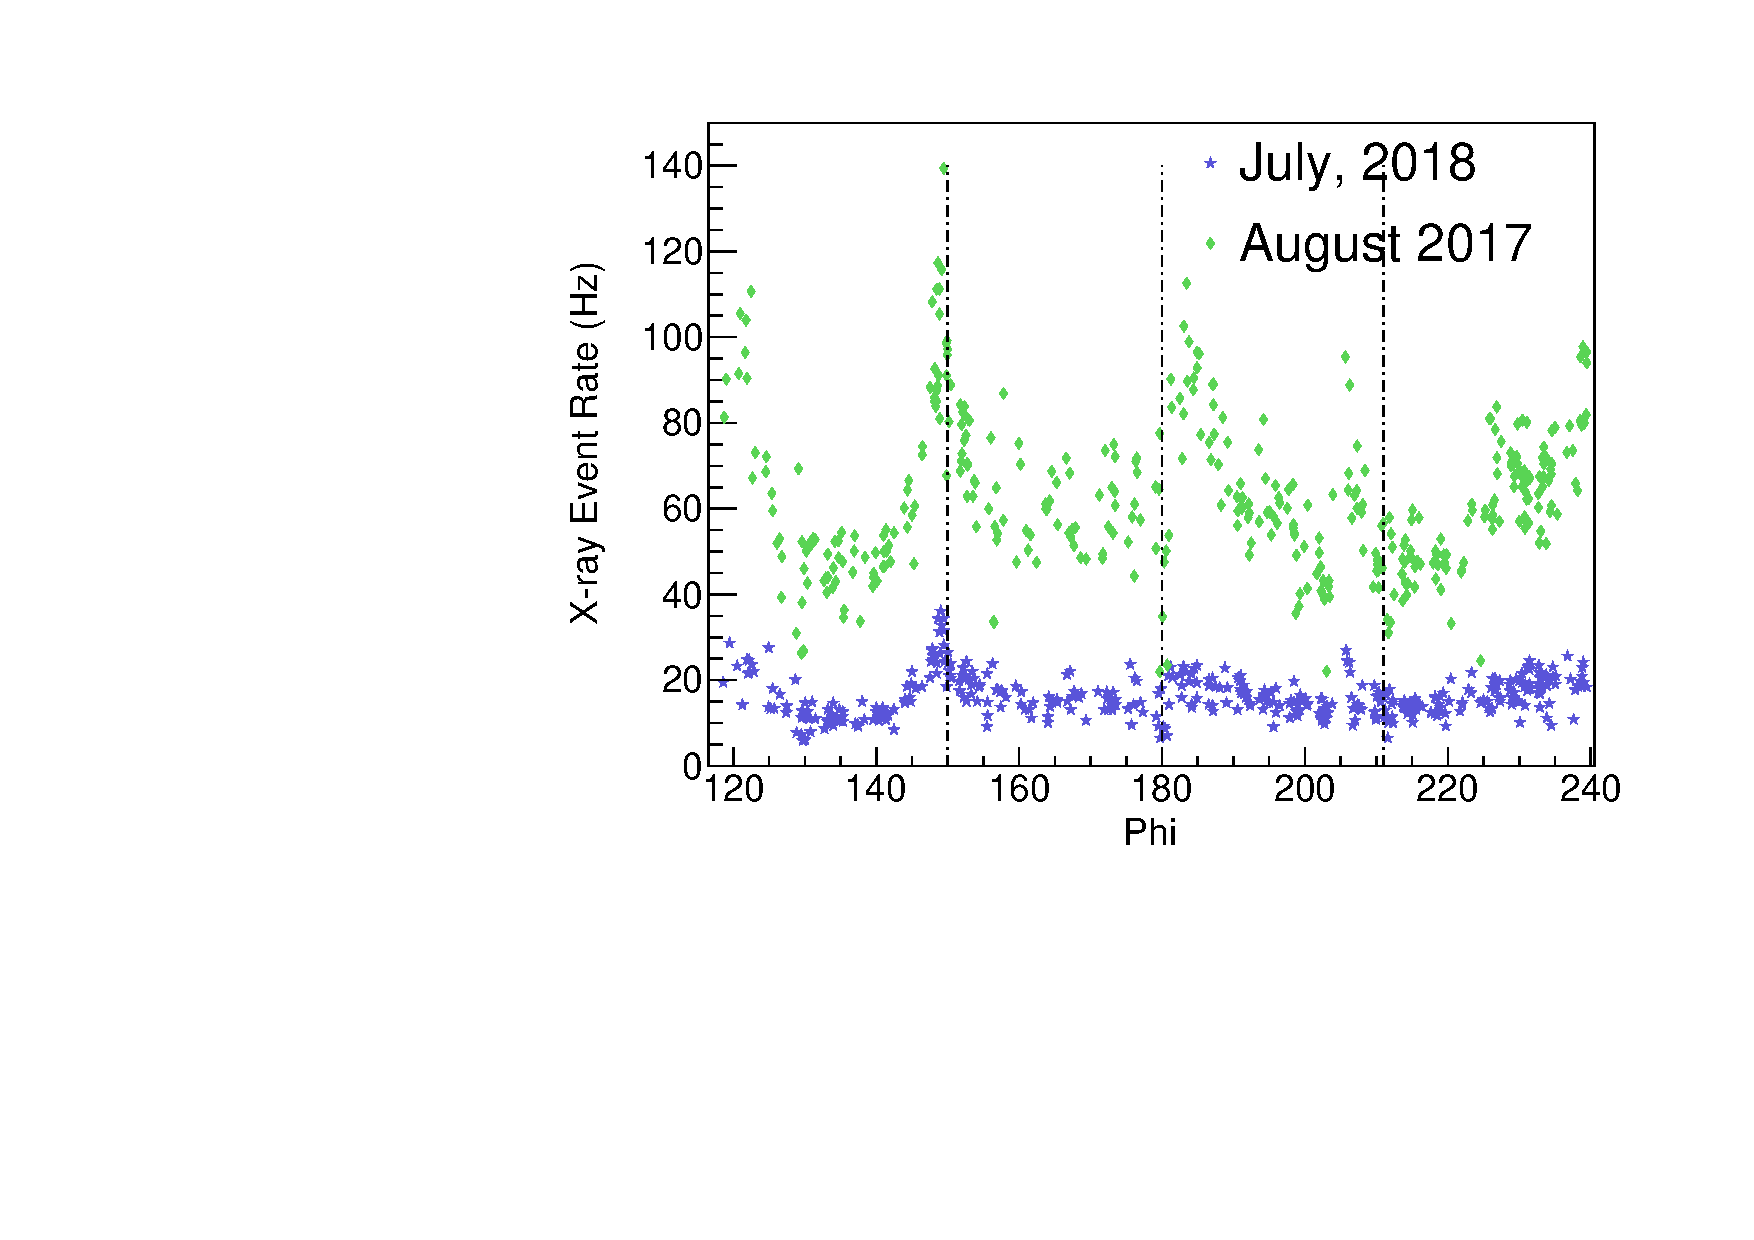
\includegraphics[width=4cm]{plots/2018/cEventRate_1718}
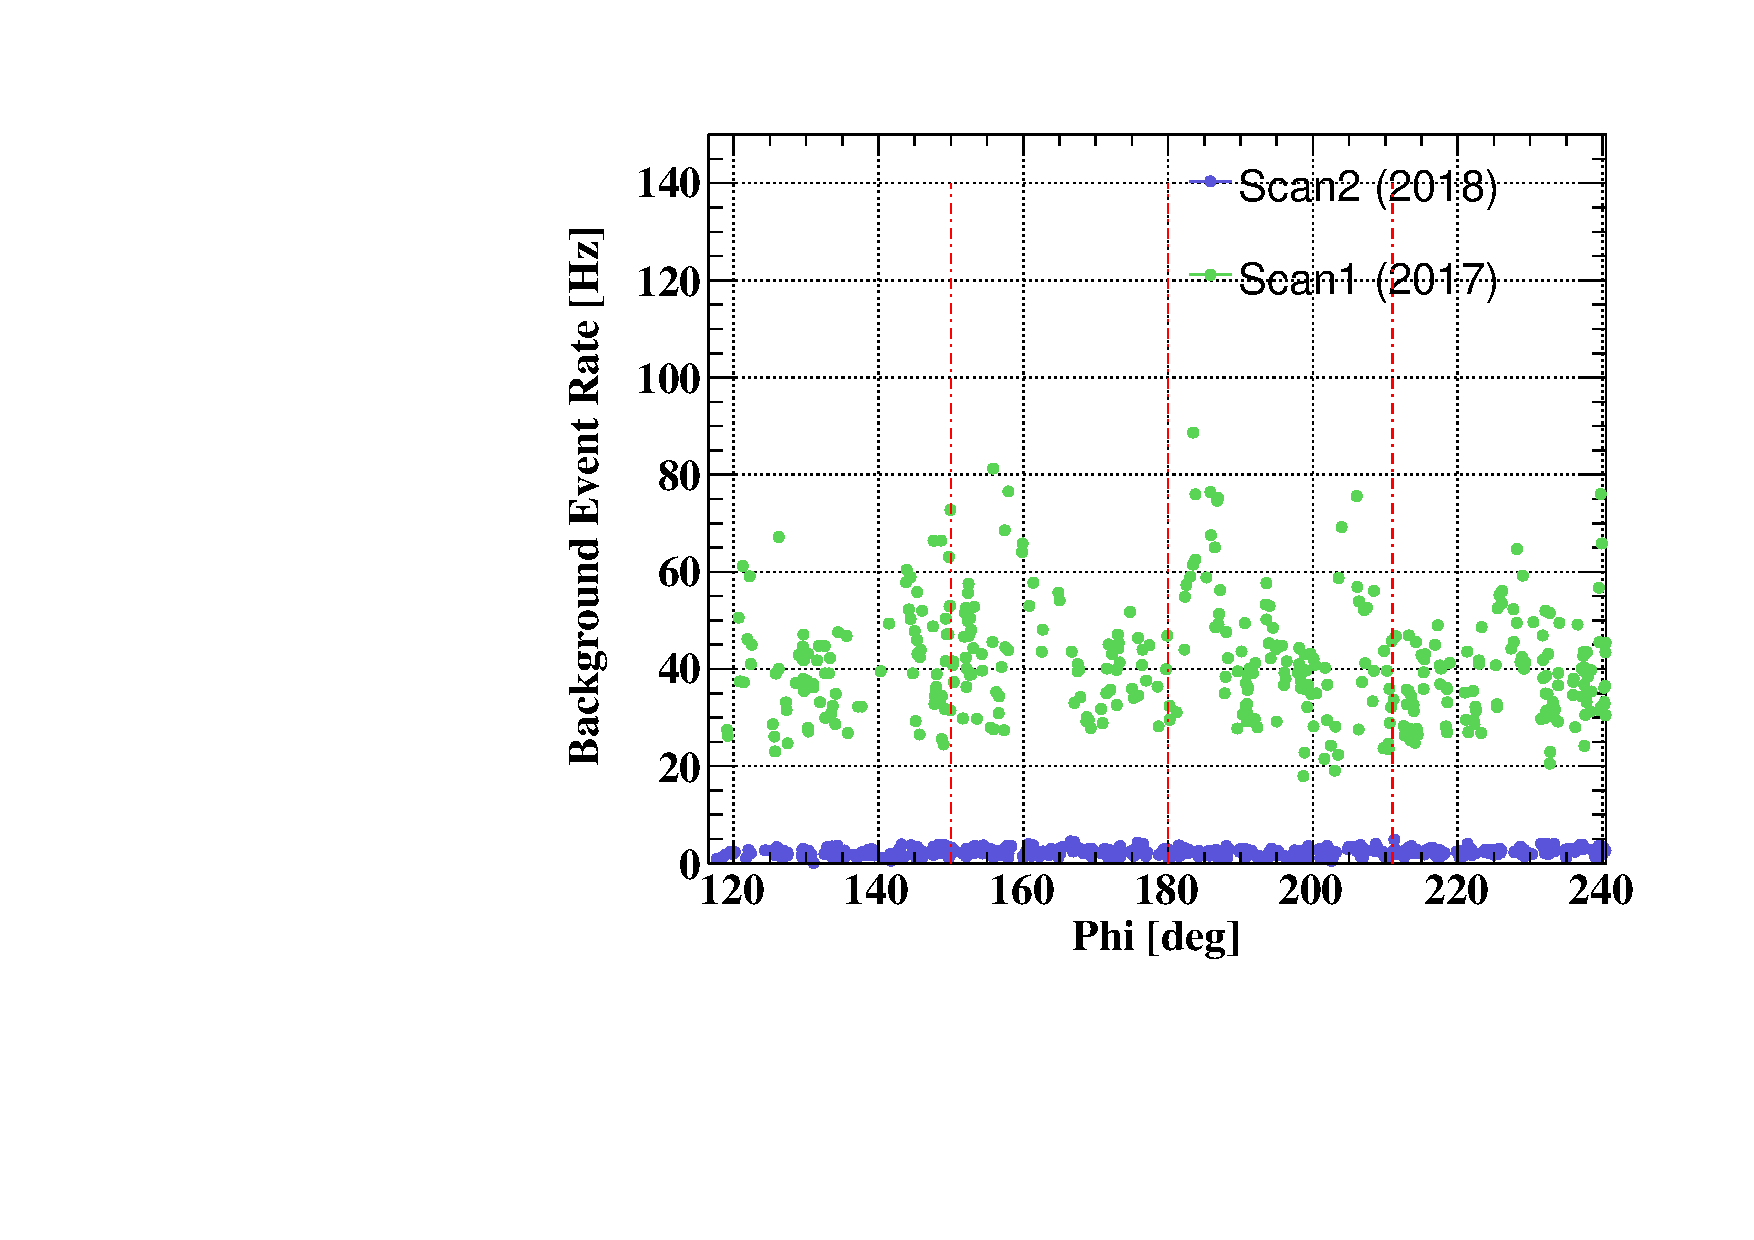
\includegraphics[width=4cm]{plots/2018/cBkgRate_1718} \\
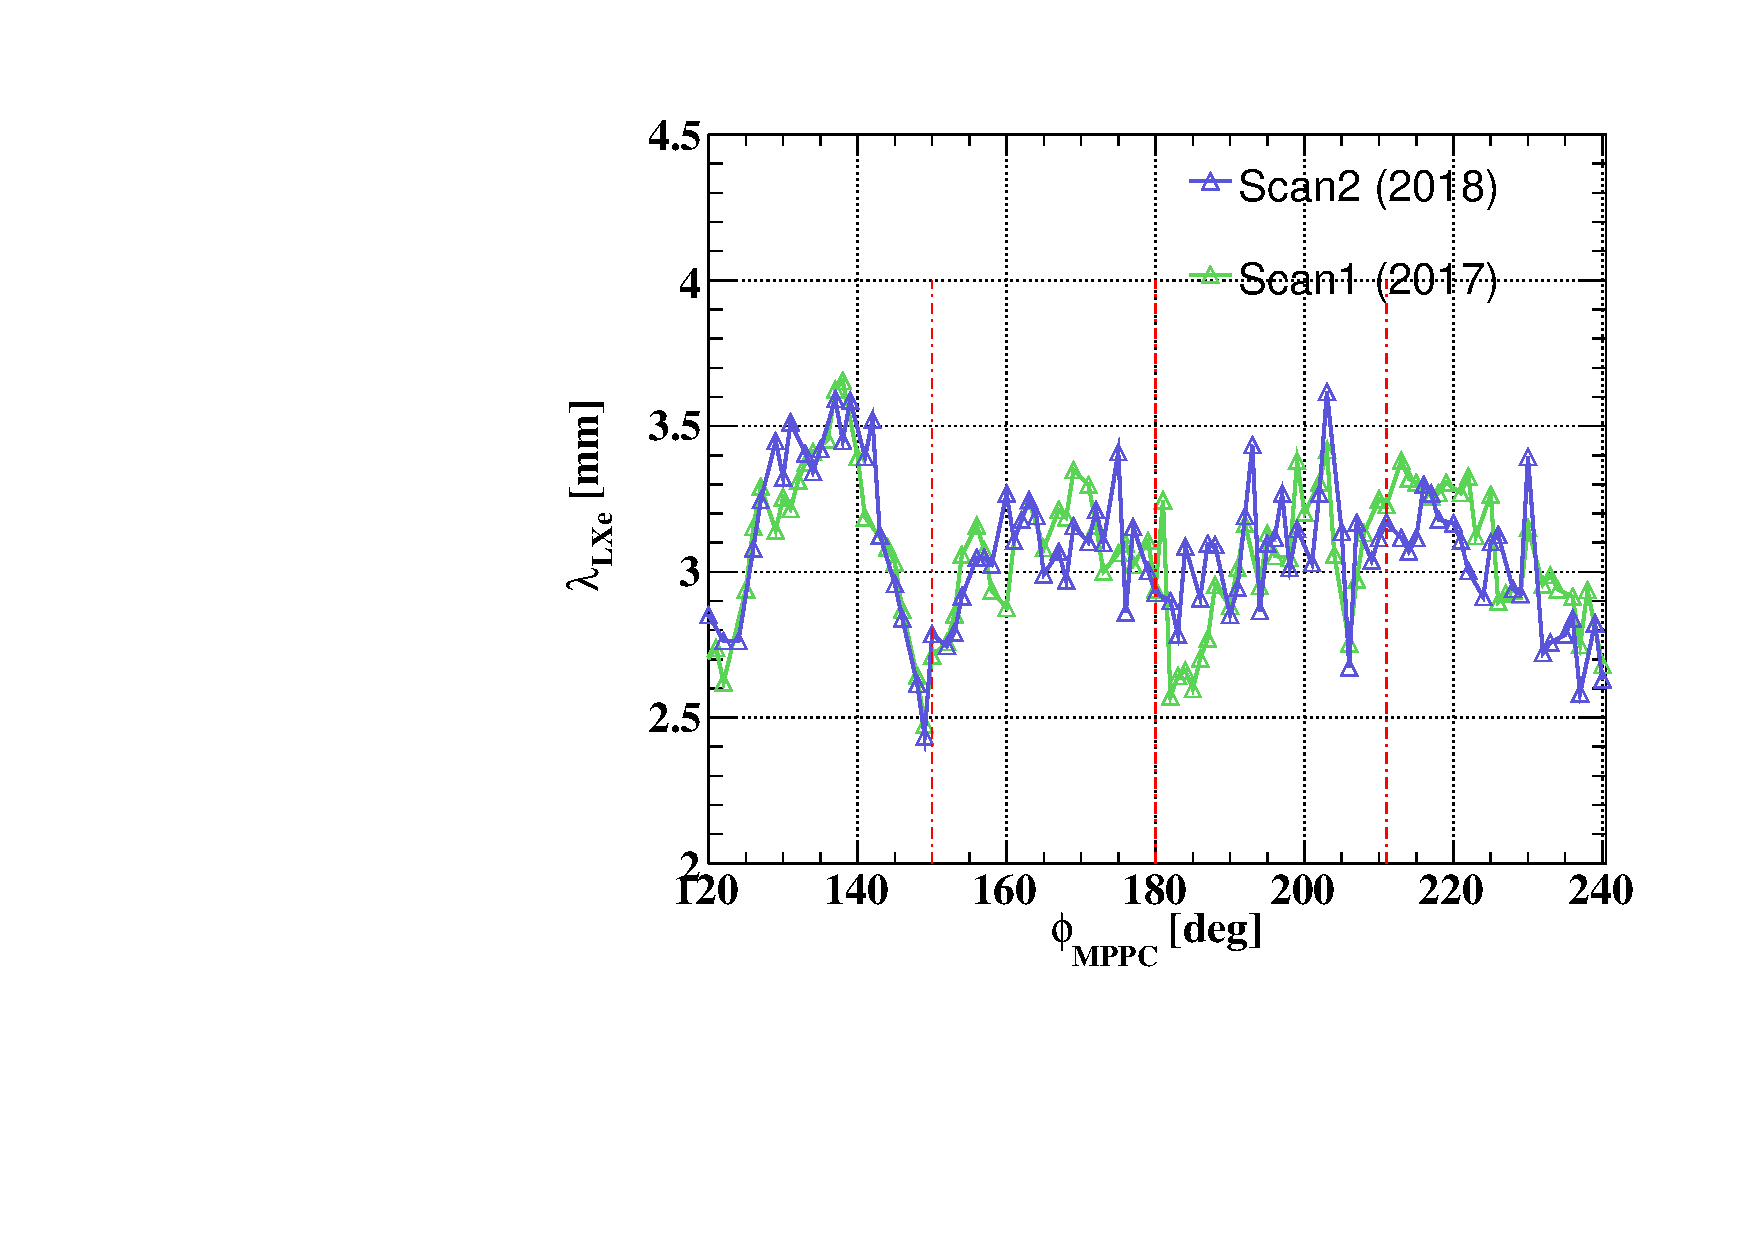
\includegraphics[width=4cm]{plots/2018/AbsorptionLength} 
\caption{Signal and background trigger rates observed in MPPC as a function of $\phi$.
Red dashed lines indicate the edges of the CFRP plate.}
\label{fig:ratesvszphi} \end{figure}


\subsection{Quantum Efficiency$\times$Gain}\label{sec:qegain}
\begin{comment}



\textbf{ADD REFERENCE TO SECTION3: MPPC STRUCTURE, CALORIMETER, 
SECTION6: INITIAL MPPC SCAN}\\
\end{comment}
In this section, we discuss our found charge gains between the individual MPPCs and between the four production batches in which we sourced the MPPCs.

Utilizing the collimated X-ray beam as a uniform light source, the mean charge
response is measured across the 12mm face of individual mppcs 
%, proportional to the gain and quantum efficiency, 
 The mean charge response
then serves as a measure of the relative gain$\times$QE between photodetectors
in the scanned region of the calorimeter. % It must be noted
%that the charge measurement contains smaller but inseparable
%contributions from after-pulse and cross-talk between neighboring
%photodetectors, which are independent from the photodetector gain.
Only relative measurements of gain are possible as the
absolute photon yield in the X-ray interaction relies on other factors
such as presence of impurities in the liquid Xenon which were not
precisely known. 

\begin{comment}
The photodetectors are developed according to the experimental
requirements with large photosensitive area 12 $\times$ 12 mm$^2$,
comprised of four  smaller pixels 6 $\times$ 6 mm$^2$ connected in
series.  The photodetectors are placed in a ceramic case (15 mm) and
mounted on a PCB strip, each containing 22 photodetectors.  Two
identically produced strips aligned along $\hat{z}$ direction, and
rotated by 180\degree with respect to each other to allow for
electronics readout at each end, make up a single row (fig 
\ref{fig:mppc}).
\end{comment}

%The mean charge  is calculated over the 12 mm region centered at the
%fitted photodetector location from previous analysis.  Due to long
To reduce the impact of high energy tails
in the charge distribution, the mean is measured using an iterative Gaussian fit; the
initial fit covers the entire range and then the fit range is restricted to the two sigma
region of the first fit.  Fig. \ref{fig:mppccharge} shows these mean charges vary overall between the
scanned photodetectors by 50\%, and correlate reliably with the
production batch of the photodetectors (fig \ref{fig:mppccharge}). 

\begin{figure}
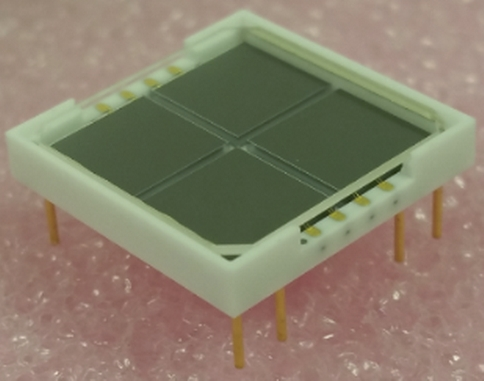
\includegraphics[width=3cm]{plots/single_mppc.jpg}
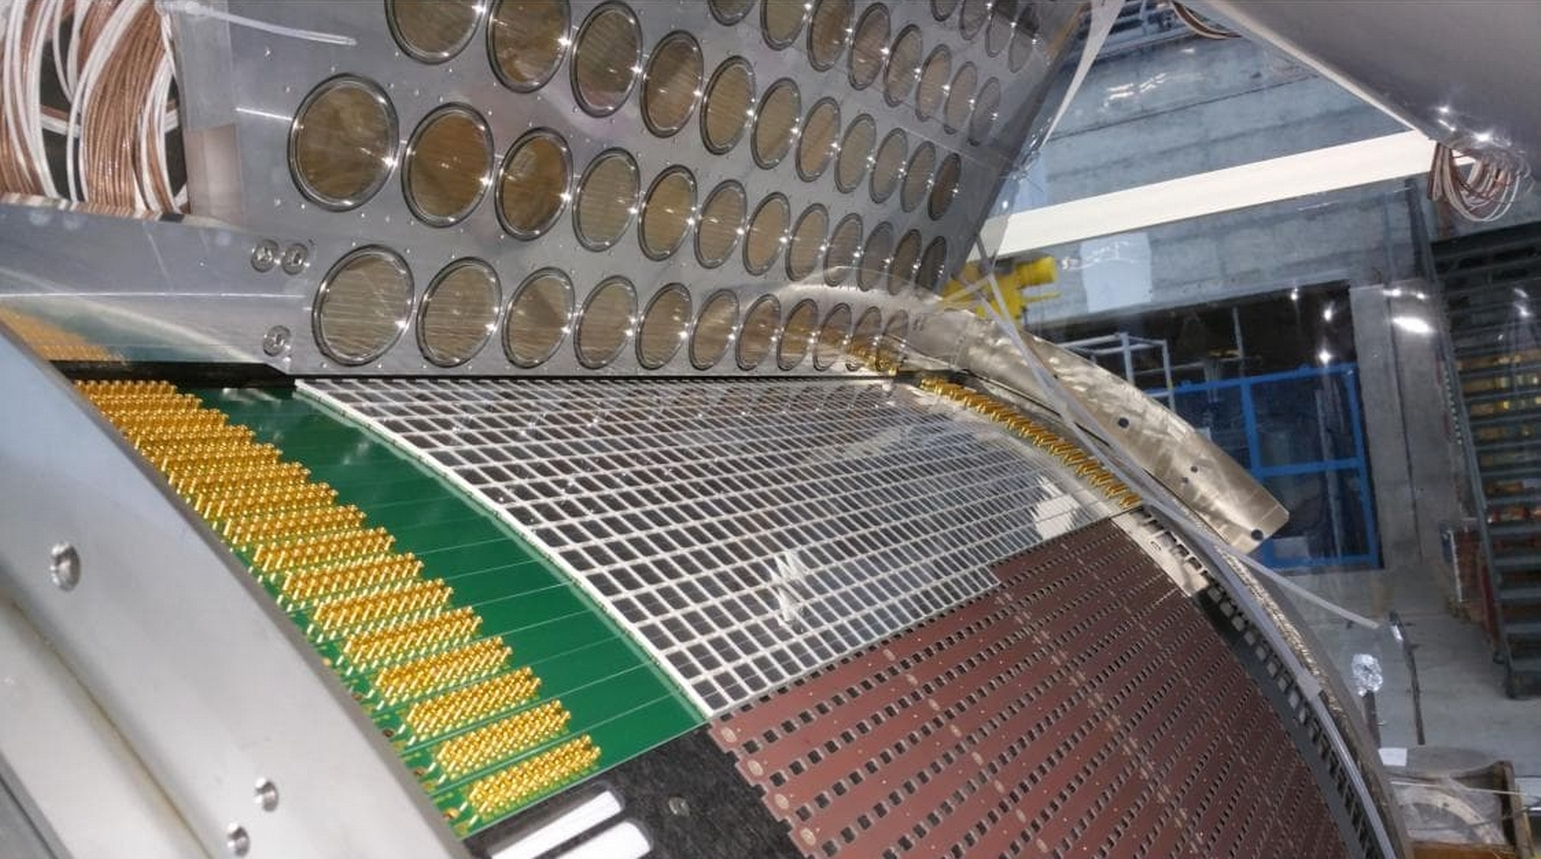
\includegraphics[width=5cm]{plots/CFRP_spacer_MPPC.jpg}
\caption{Single MPPC and installed MPPCs in the LXe calorimeter.}
\label{fig:mppc} 
\end{figure}

\begin{figure}
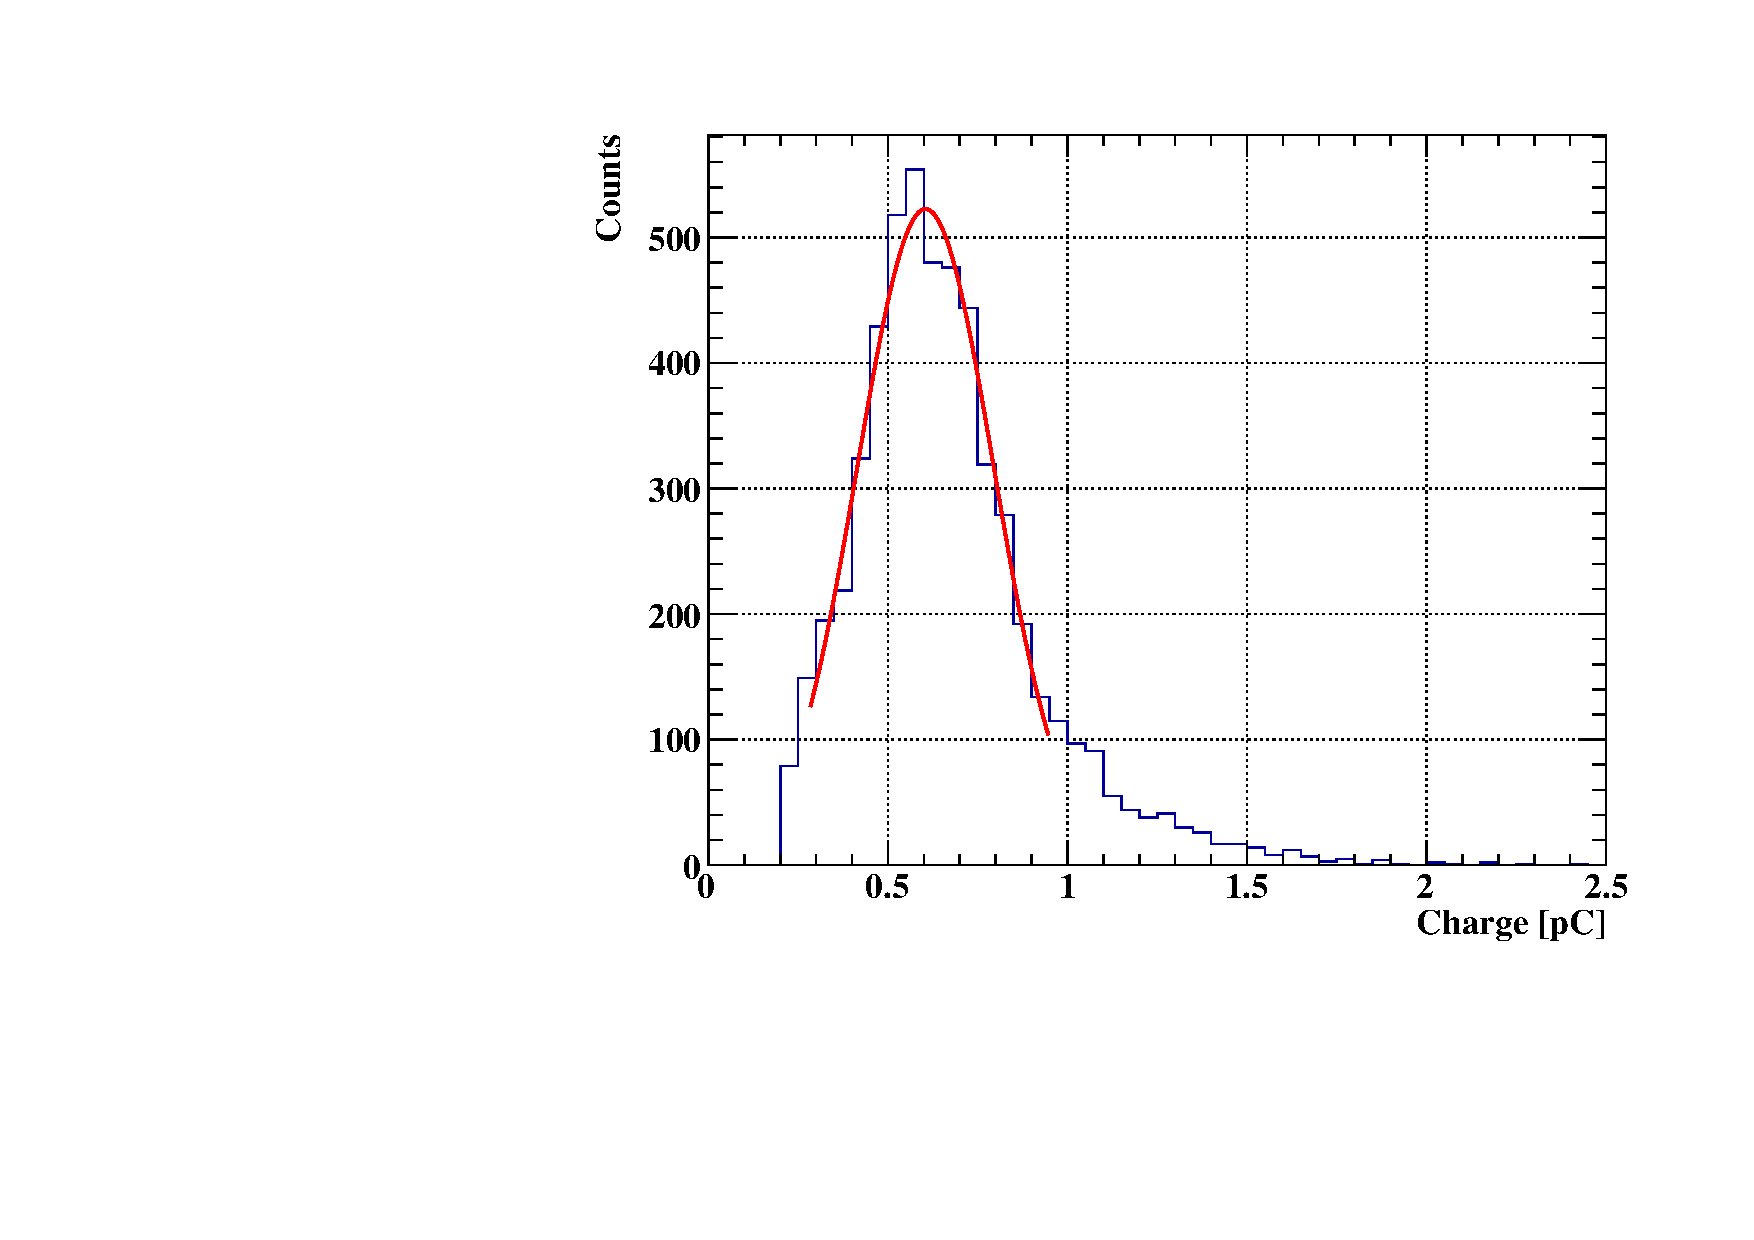
\includegraphics[width=4cm]{graphics/q64fit.pdf}
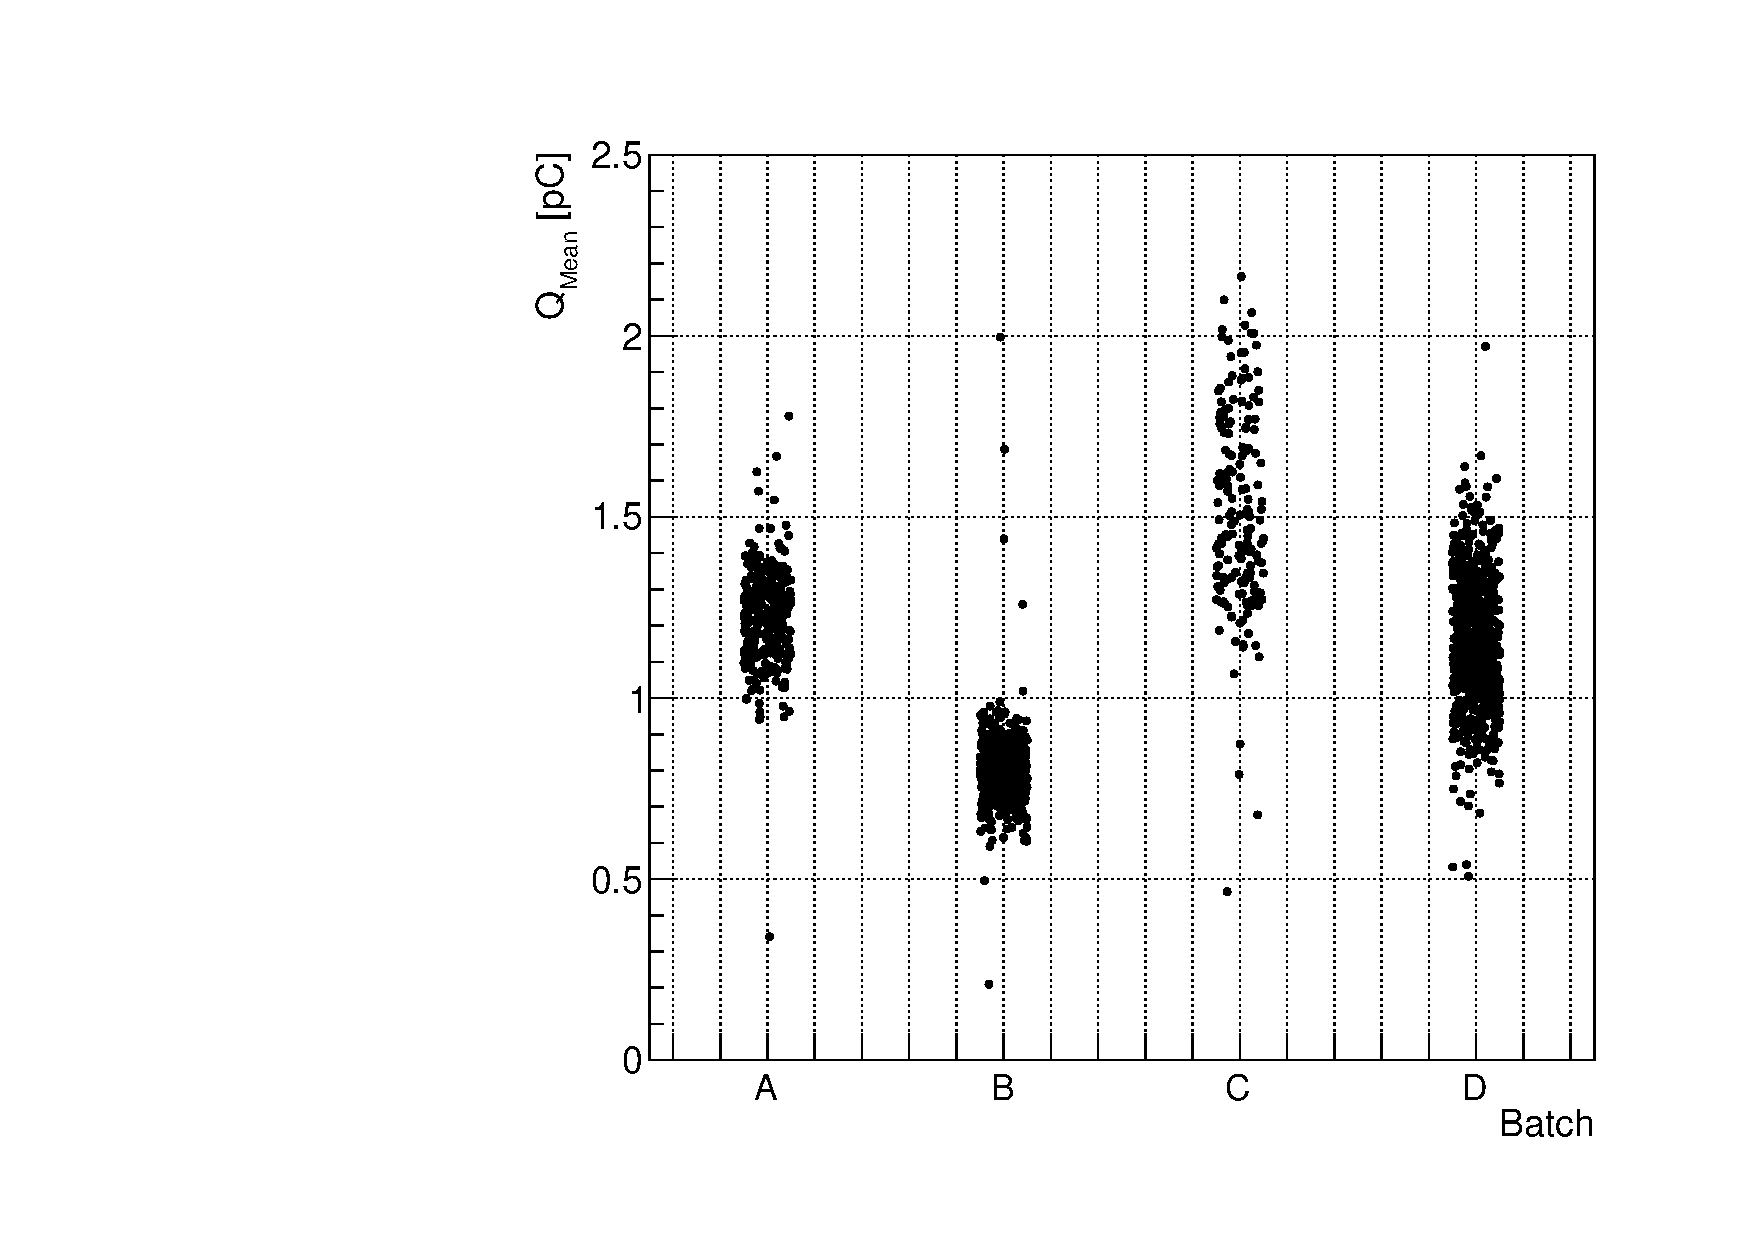
\includegraphics[width=4cm]{plots/2018/qmean_vs_batch.pdf}
\caption{Charge measured in a single MPPC with gaussian fit (left).
Mean charge measured measured in the batch (right). }
\label{fig:mppccharge} 
\end{figure}


\subsection{Sub-MPPC/Quadrant Gain}
Furthermore, we describe here variations in gain across the active area of individual photodetectors.

The fine scanning resolution (scanning step 1 mm in z and \phis, and
X-ray beam size  $\sim$ 1 mm), is used to determine variation in
charge response of the component pixels of the photodetector.  The
position dependent variation in mean charge seen in figure
\ref{fig:xrayevents} demonstrates the difference in the response of
half photodetector  (two of four pixels) illuminated at every
position.  A visible decrease at the center of the photodetector is
caused by the central gap between the two rows of pixels.  Mean charge
in each half of the photodetector is independently calculated about
the center position determined in the previous analysis.  We find that
the mean charge varies between the two halves seperated by their Z
coordinate by 10\% and equal in the two halves separated by \phis.  Due
to the relative rotation the PCB strips per row about the center, the
mean charge of each half of the photodetector is also swapped
accordingly (fig \ref{fig:pixelcharge}). 
This disparity in charge response
is found to be independent of the production batch of the 
photodetector, observed at consistent level across all
batch groups.

\begin{figure}
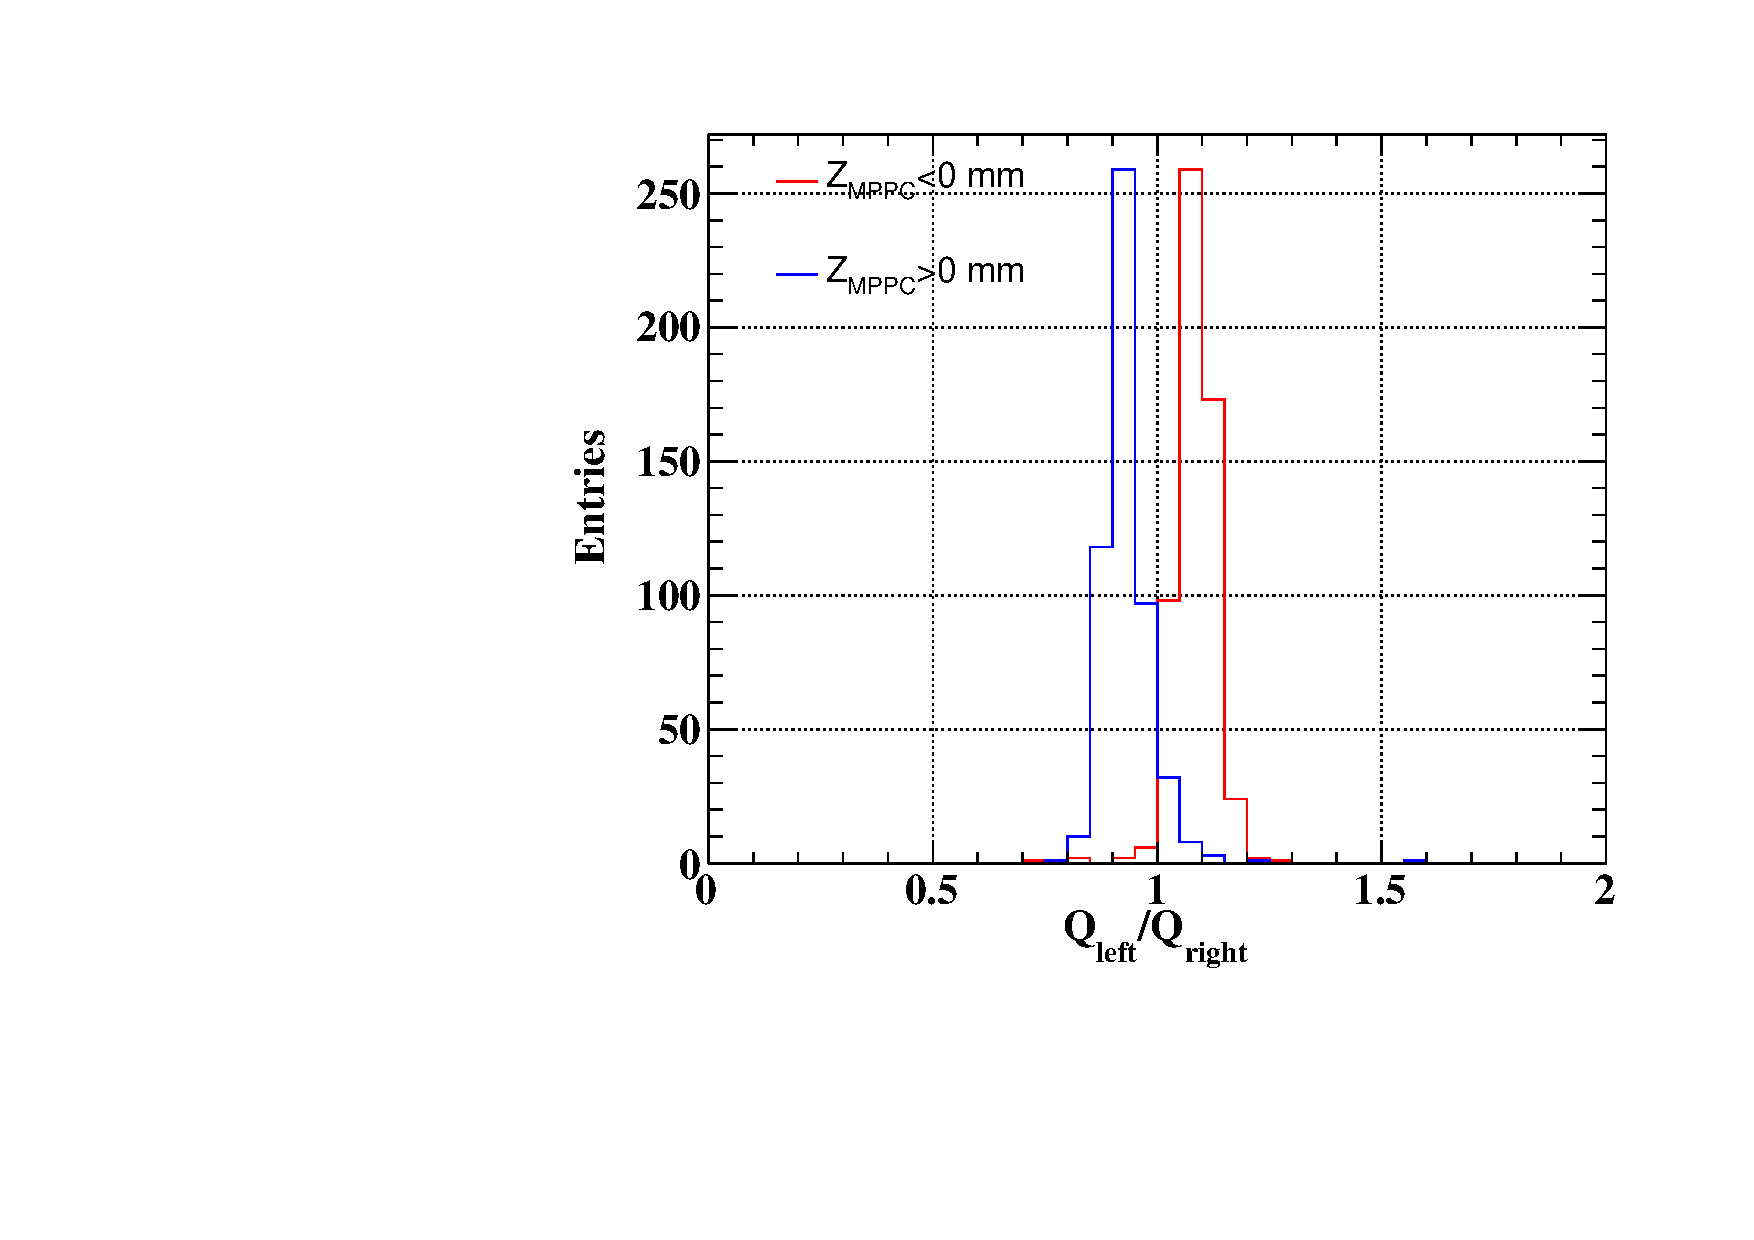
\includegraphics[width=4cm]{plots/2018/qratio_z_wf.pdf}
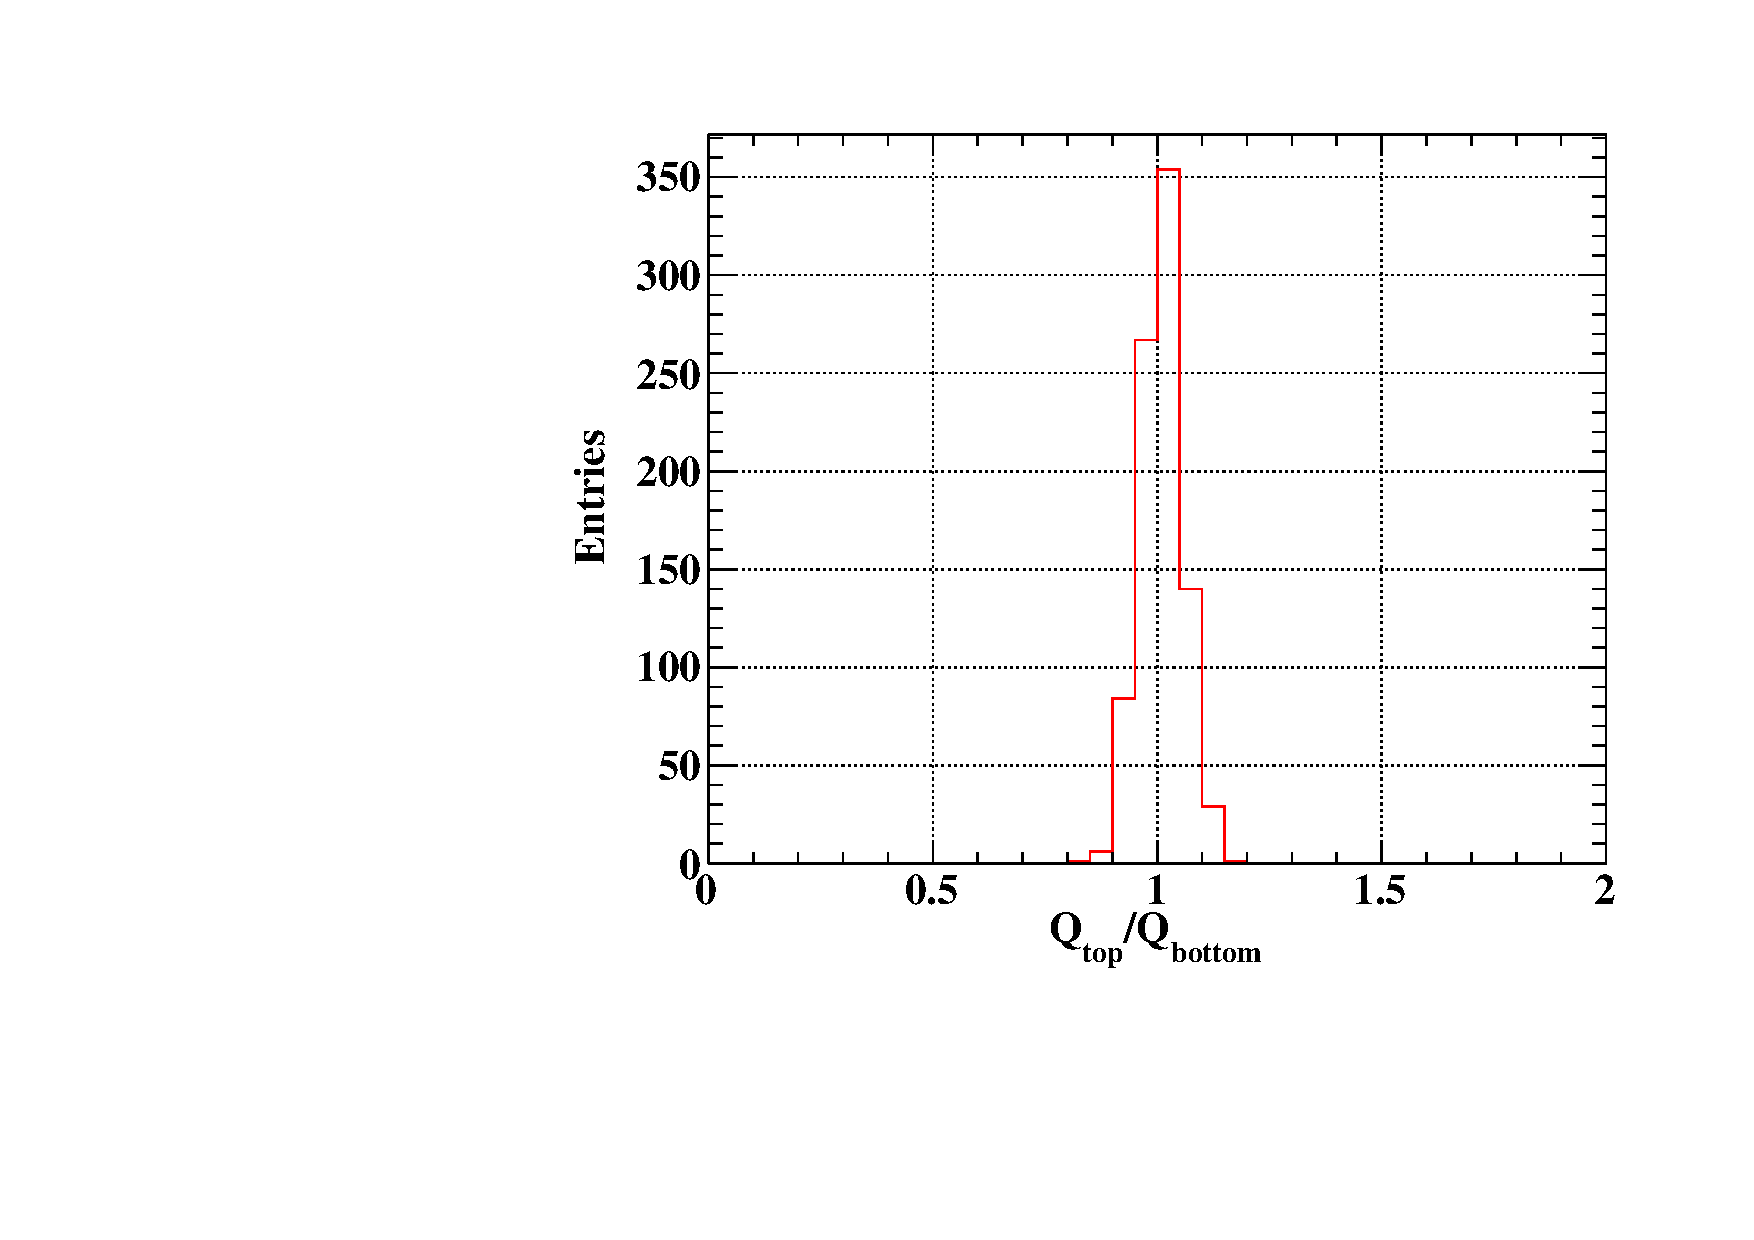
\includegraphics[width=4cm]{plots/2018/qratio_phi_wf.pdf}
\caption{Relative mean charge the two halves of the 
photodetectors in the scanning direction.}
\label{fig:pixelcharge} 
\end{figure}





